\section{Timeline}
A timeline for this semester can be seen in figure 3 there are a significant amount of tasks that overlap. In some cases it could be seen that there are also very few tasks for november. Both of these observations are due to the fact that the PicoBalloon is highly affected by weather and the fact that future work on the PicoBalloon is based on how the second test goes in october, weather prevailing.
\begin{figure}[H]
    \begin{center}
            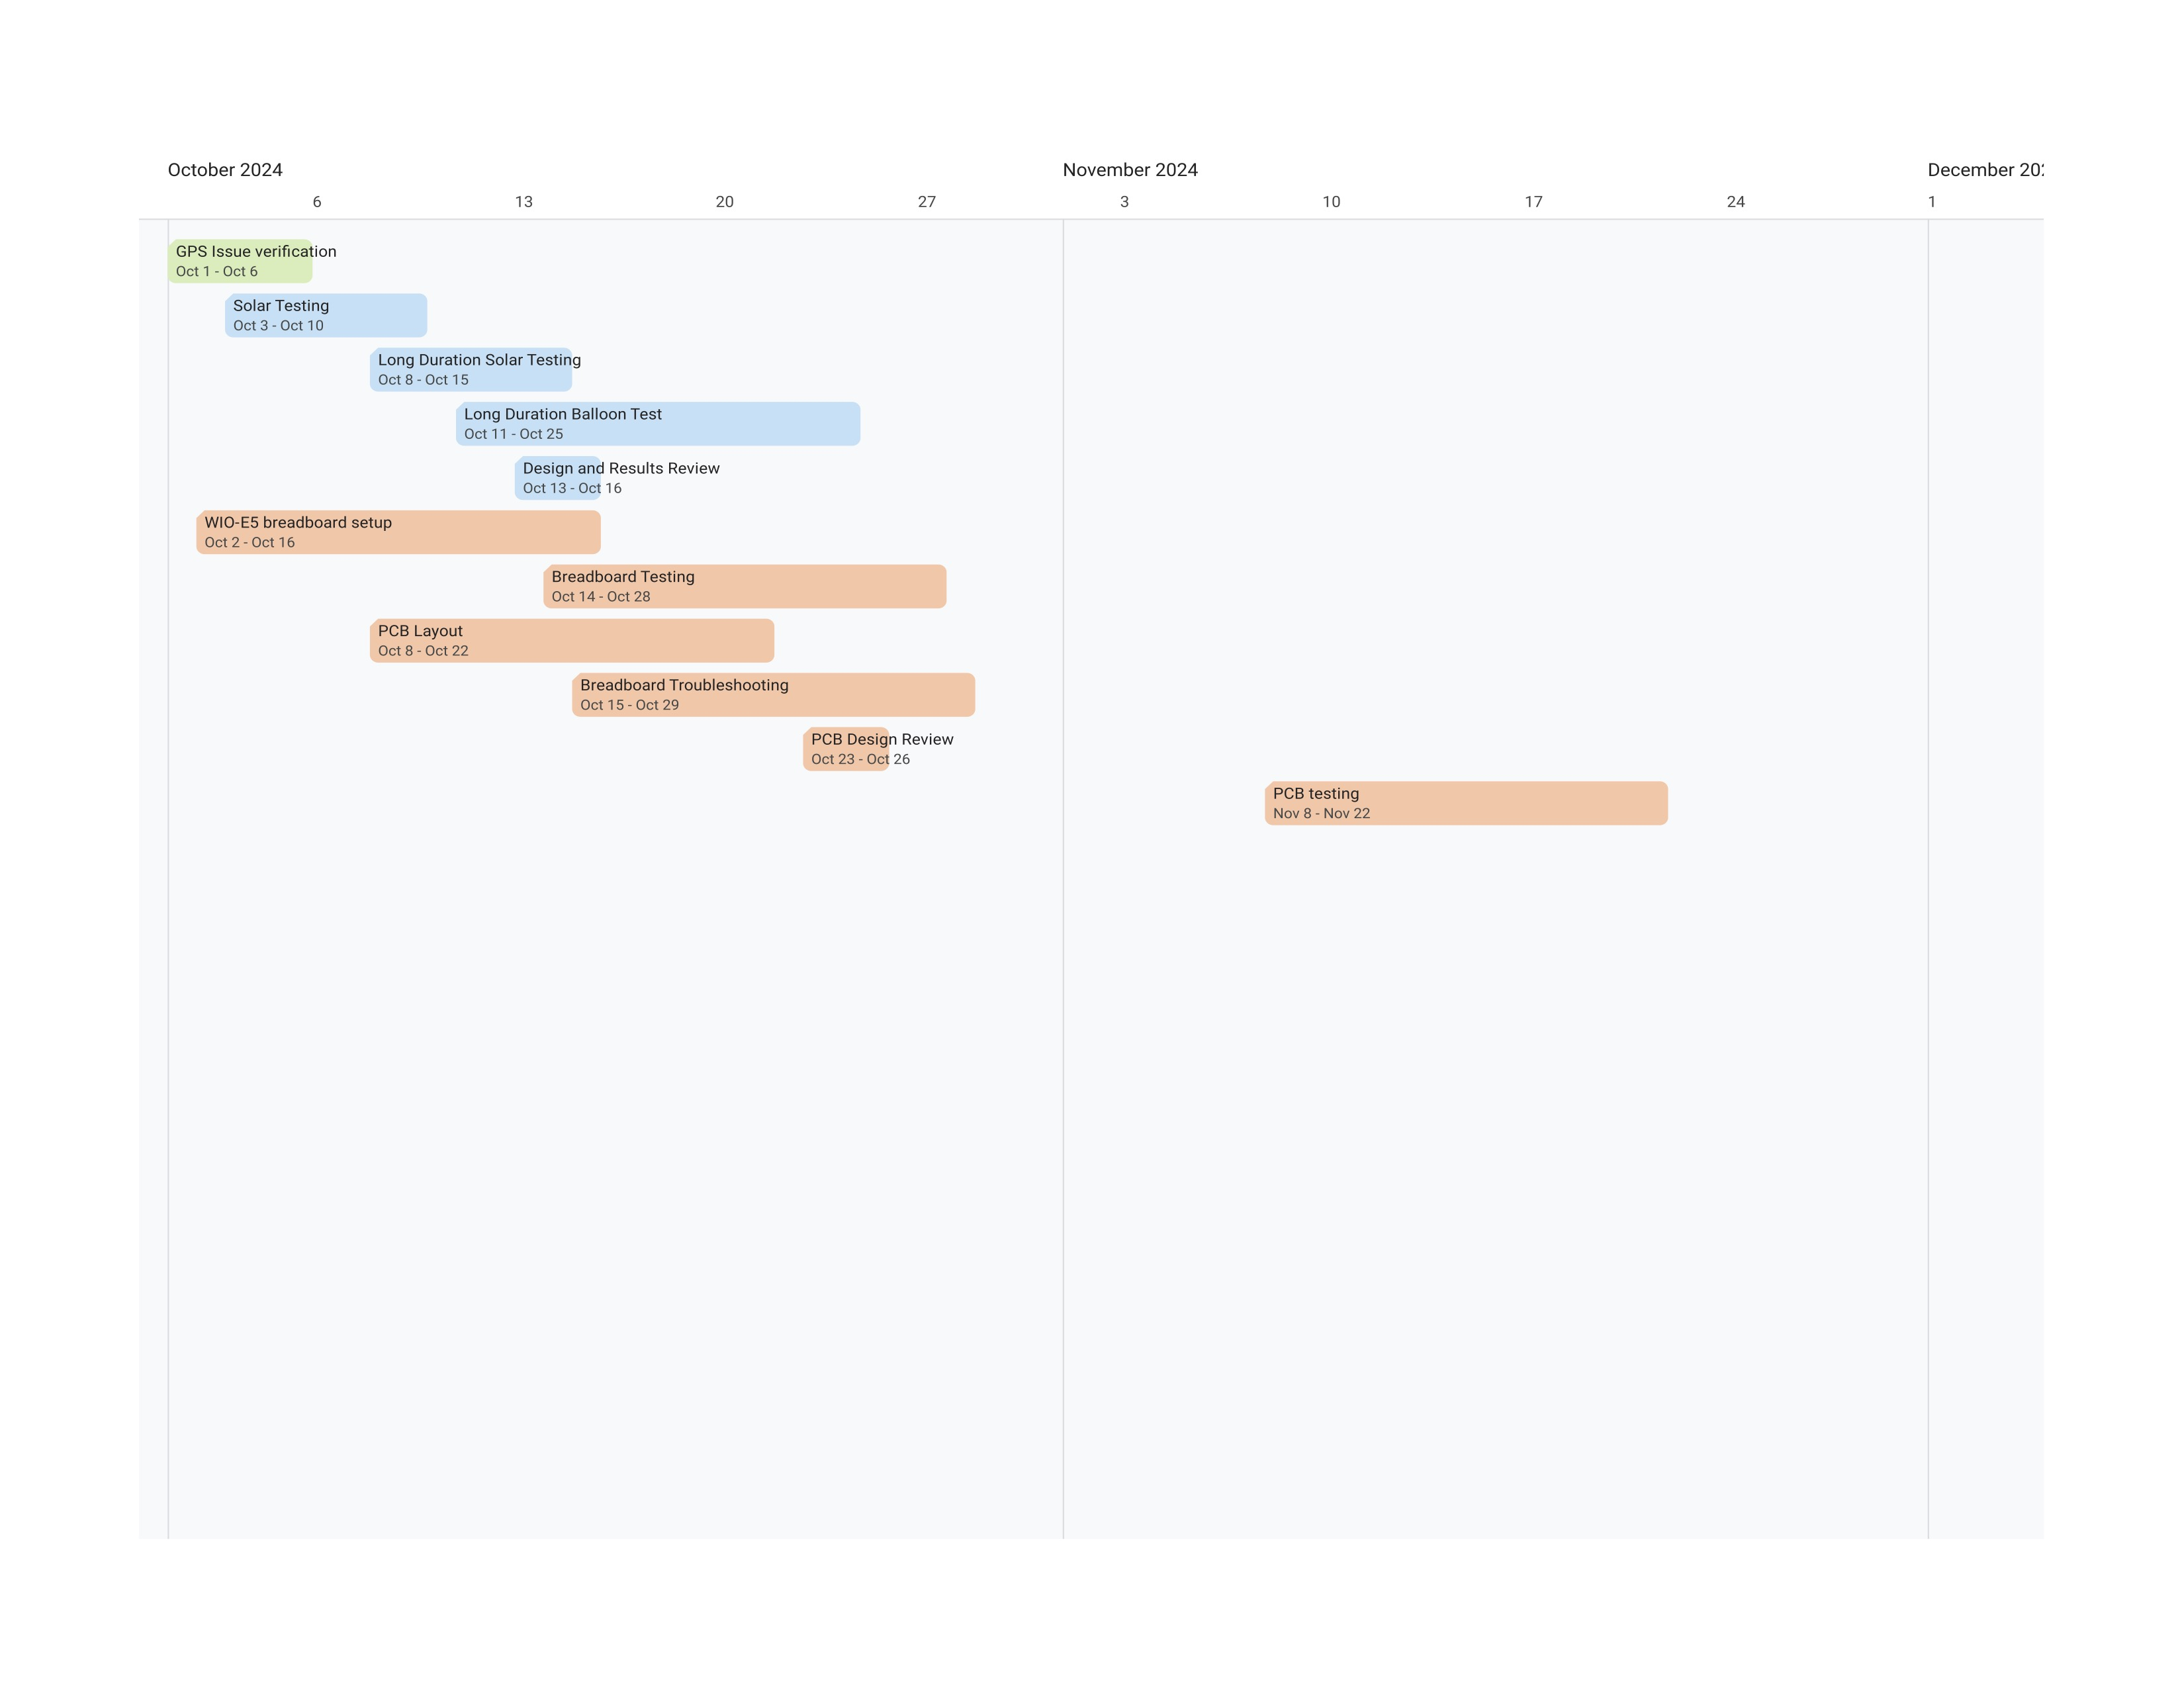
\includegraphics[width=1\textwidth]{Images/SSDS Timeline.jpg}\caption{A (mostly) semester long timeline for SSDS work}
    \end{center}
\end{figure}
The DeSCENT mission tasks are all in orange, these tasks are on a rolling timeline essentially as some of them are sequential, and V2 is not the main priority. The launch window could open as soon as november, so working out any issues with the V1 is crucial  before then. If the focus this semester becomes solely V1 then V2 will be the focus of next semester. Figure 3 is difficult to read so here is the data that went into the chart
\begin{table}[!htp]\centering
    \scriptsize
    \begin{tabular}{lrr}\toprule
        Task &Duration(days) \\\cmidrule{1-2}
        GPS Issue verification &5 \\
        Solar Testing &7 \\
        Long Duration Solar Testing &7 \\
        Long Duration Balloon Test &14 \\
        Design and Results Review &3 \\
        WIO-E5 breadboard setup &21 \\
        Breadboard Testing &21 \\
        PCB Layout &14 \\
        Breadboard Troubleshooting &21 \\
        PCB Design Review &3 \\
        PCB testing &14 \\
        \bottomrule
    \end{tabular}
\end{table}
Moving into the next semester will consist majorly of testing the V2 chipsat, which is beginning to be ordered as of now -- Nov 2024. Given that this project is research based I originally left out next semester from the timeline because it would be heavily based on what occured this semester. This semester has been filled with more issues than wins on the picoballoon chip sats and the v2 mcu, less progress than initially intended has been achieved. This actually works out well on a project basis as it leaves a significant amount of work for the V2 chipsat in semester 2.